% One step of the sweeping algorithm (notebook 56, Section 6).
% (a) the bond tensor B^l of sites j, j+1 (the label leg sits on it);
% (b) the projected input of image n: the left and right environments L_n, R_n of the data and the two feature vectors;
% (c) the SVD split with truncation to chi values; moving right, the label leg moves to site j+1.
\documentclass[tikz,border=6pt]{standalone}
\usepackage{amsmath,amssymb}
\usetikzlibrary{positioning,calc}
\tikzset{site/.style={circle, draw, thick, fill=blue!12, minimum size=0.82cm, inner sep=0pt, font=\scriptsize},
         bond/.style={rounded corners=3pt, draw, thick, fill=orange!35, minimum width=1.7cm, minimum height=0.62cm, font=\scriptsize},
         env/.style={rectangle, draw, thick, fill=green!18, minimum width=0.55cm, minimum height=0.62cm, font=\scriptsize},
         feat/.style={circle, draw, thick, fill=red!20, minimum size=0.5cm, inner sep=0pt, font=\scriptsize}}
\begin{document}
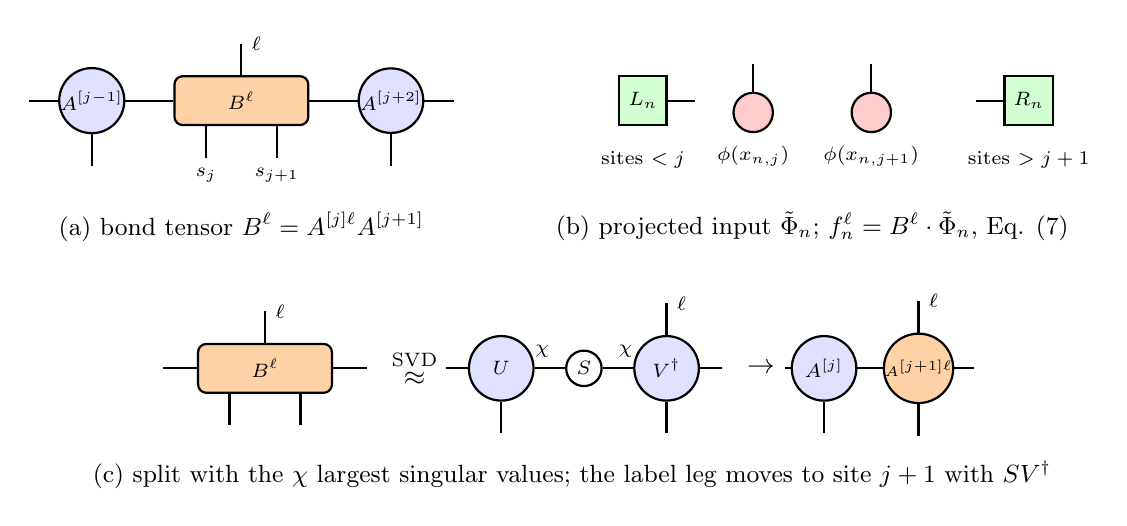
\begin{tikzpicture}
  % ------------------------------------------------------------- (a) bond tensor
  \begin{scope}[shift={(0,0)}]
    \node[site] (l1) at (0,0) {$A^{[j-1]}$};
    \node[bond] (B) at (1.9,0) {$B^{\ell}$};
    \node[site] (r1) at (3.8,0) {$A^{[j+2]}$};
    \draw[thick] (-0.8,0) -- (l1) -- (B) -- (r1) -- (4.6,0);
    \draw[thick] (l1.south) -- ++(0,-0.4); \draw[thick] (r1.south) -- ++(0,-0.4);
    \draw[thick] ($(B.south)+(-0.45,0)$) -- ++(0,-0.4) node[below, font=\scriptsize] {$s_j$};
    \draw[thick] ($(B.south)+(0.45,0)$) -- ++(0,-0.4) node[below, font=\scriptsize] {$s_{j+1}$};
    \draw[thick] (B.north) -- ++(0,0.4) node[right, font=\scriptsize] {$\ell$};
    \node[font=\small, align=center] at (1.9,-1.6) {(a) bond tensor $B^{\ell}=A^{[j]\ell}A^{[j+1]}$};
  \end{scope}
  % ------------------------------------------------------------- (b) projected input
  \begin{scope}[shift={(7.0,0)}]
    \node[env] (L) at (0,0) {$L_n$};
    \node[feat] (p1) at (1.4,-0.15) {}; \node[feat] (p2) at (2.9,-0.15) {};
    \node[env] (R) at (4.9,0) {$R_n$};
    \draw[thick] (L.east) -- ++(0.35,0); \draw[thick] (R.west) -- ++(-0.35,0);
    \draw[thick] (p1.north) -- ++(0,0.35); \draw[thick] (p2.north) -- ++(0,0.35);
    \node[font=\scriptsize] at (1.4,-0.7) {$\phi(x_{n,j})$}; \node[font=\scriptsize] at (2.9,-0.7) {$\phi(x_{n,j+1})$};
    \node[font=\scriptsize, align=center] at (0,-0.75) {sites $<j$};
    \node[font=\scriptsize, align=center] at (4.9,-0.75) {sites $>j+1$};
    \node[font=\small, align=center] at (2.15,-1.6) {(b) projected input $\tilde\Phi_n$; $f^{\ell}_n=B^{\ell}\cdot\tilde\Phi_n$, Eq. (7)};
  \end{scope}
  % ------------------------------------------------------------- (c) SVD split
  \begin{scope}[shift={(2.2,-3.4)}]
    \node[bond] (B2) at (0,0) {$B^{\ell}$};
    \draw[thick] (-1.3,0) -- (B2) -- (1.3,0);
    \draw[thick] ($(B2.south)+(-0.45,0)$) -- ++(0,-0.4); \draw[thick] ($(B2.south)+(0.45,0)$) -- ++(0,-0.4);
    \draw[thick] (B2.north) -- ++(0,0.4) node[right, font=\scriptsize] {$\ell$};
    \node at (1.9,0) {$\overset{\rm SVD}{\approx}$};
    \node[site] (U) at (3.0,0) {$U$};
    \node[circle, draw, thick, fill=white, minimum size=0.45cm, inner sep=0pt, font=\scriptsize] (S) at (4.05,0) {$S$};
    \node[site] (V) at (5.1,0) {$V^{\dagger}$};
    \draw[thick] (2.3,0) -- (U) -- (S) -- (V) -- (5.8,0);
    \draw[thick] (U.south) -- ++(0,-0.4); \draw[thick] (V.south) -- ++(0,-0.4);
    \draw[thick] (V.north) -- ++(0,0.4) node[right, font=\scriptsize] {$\ell$};
    \node[font=\scriptsize] at (3.52,0.22) {$\chi$}; \node[font=\scriptsize] at (4.58,0.22) {$\chi$};
    \node at (6.3,0) {$\to$};
    \node[site] (A1) at (7.1,0) {$A^{[j]}$};
    \node[site, fill=orange!35] (A2) at (8.3,0) {\tiny$A^{[j+1]\ell}$};
    \draw[thick] (6.6,0) -- (A1) -- (A2) -- (9.0,0);
    \draw[thick] (A1.south) -- ++(0,-0.4); \draw[thick] (A2.south) -- ++(0,-0.4);
    \draw[thick] (A2.north) -- ++(0,0.4) node[right, font=\scriptsize] {$\ell$};
    \node[font=\small, align=center] at (3.9,-1.35) {(c) split with the $\chi$ largest singular values; the label leg moves to site $j+1$ with $SV^{\dagger}$};
  \end{scope}
\end{tikzpicture}
\end{document}
